\documentclass[11pt]{article}

\usepackage[a4paper,margin=2cm]{geometry}
\usepackage{fontspec}
\setmainfont{texgyrepagella}[
  Extension = .otf,
  UprightFont = *-regular,
  BoldFont = *-bold,
  ItalicFont = *-italic,
  BoldItalicFont = *-bolditalic]
\usepackage{microtype}
\usepackage{graphicx}
\usepackage[skip=4pt,font=small,labelfont=bf]{caption}
\usepackage{titlesec}
\titleformat{\section}{\large\bfseries}{}{0pt}{}
\titlespacing{\section}{0pt}{14pt}{6pt}
\titleformat{\subsection}{\normalsize\bfseries\itshape}{}{0pt}{}
\titlespacing{\subsection}{0pt}{10pt}{4pt}
\usepackage{xcolor}
\definecolor{linkblue}{RGB}{25,60,120}
\usepackage[colorlinks=true,allcolors=linkblue]{hyperref}
\usepackage{parskip}
\setlength{\parskip}{4pt}

\pagestyle{plain}

\begin{document}

\begin{center}
  {\LARGE\bfseries Research Statement}\\[6pt]
  {\large Chunlei Li}\\[2pt]
  Ph.D.\ Candidate, Beihang University \,·\, Visiting Ph.D.\ Student, University College London\\
  \href{https://chunleili.github.io/}{chunleili.github.io} \,·\, \href{mailto:lichunlei1996@gmail.com}{lichunlei1996@gmail.com} \,·\, \href{mailto:li_cl@foxmail.com}{li\_cl@foxmail.com}\\[3pt]
  July 2026
\end{center}

\section{Overview}

My research goal is to build physical simulators that are fast, robust, and scalable enough to be trusted as infrastructure: for animation, for biomechanics, and as data engines and differentiable layers for machine learning. I work at the interface of numerical methods and learning. On one side, I develop solvers (multigrid-accelerated XPBD, unified SPH, parallel constraint processing) that push the resolution and stiffness limits of deformable simulation. On the other, I use these simulators to train and drive learning-based systems, such as reinforcement-learning controllers for muscle-driven characters. I believe the most valuable progress in this area comes from preserving the robustness and interpretability of principled numerical simulation while letting data determine what is genuinely hard to model by hand: constitutive behavior, control policies, and model parameters. Someone has to invent and build the simulator before any data-driven layer can stand on it, and that is the role I want to keep playing.

\section{Past and Current Research}

\subsection{Robust and scalable solvers for deformable dynamics}

XPBD is the workhorse of interactive deformable simulation, but its local Gauss--Seidel iteration stalls on low-frequency error modes, exactly in the regimes that matter most: high resolution and high stiffness. In \textbf{MGPBD} (SIGGRAPH 2025) I reformulated the constraint solve as a global optimization preconditioned by unsmoothed-aggregation algebraic multigrid (UA-AMG), with lazy reuse of prolongation operators across time steps and a lightweight near-kernel construction to keep the overhead practical. The solver converges reliably where standard XPBD diverges, at a fraction of the cost of a full Newton solve.

\begin{figure}[htb]
  \centering
  \includegraphics[width=0.56\linewidth]{../images/mgpbd_preview.png}
  \caption{MGPBD enables stable, high-resolution volumetric soft-body and muscle simulation at interactive rates (SIGGRAPH 2025).}
\end{figure}

I later brought this line of work into production as multigrid-accelerated GPU muscle simulation inside Houdini at Alibaba, which taught me what practitioners actually demand from a solver: predictable behavior under bad inputs, not just good average-case performance. I also contributed to a Pacific Graphics 2025 paper on \textbf{real-time soft-body cutting}, restoring GPU solver parallelism after topology changes through on-the-fly constraint-graph re-partitioning and re-coloring. I see this as a close cousin of robust contact handling, since both destroy the static structure that fast parallel solvers rely on.

\subsection{Unified constitutive modeling of complex materials}

Materials such as mud, dough, and slime traverse fluid-like and solid-like regimes within a single animation. In my \textbf{IEEE TVCG} paper on non-Newtonian simulation I developed a unified particle-based (SPH) solver whose constitutive model smoothly spans viscous, elastic, and plastic behavior in one framework. The lasting lesson for me was about structure: a well-designed parametric constitutive space is exactly what data-driven calibration needs, since it provides interpretable parameters to fit, meaningful interpolation between regimes, and stable behavior everywhere in the parameter space.

\begin{figure}[htb]
  \centering
  \includegraphics[width=0.56\linewidth]{../images/nonNewton_preview.png}
  \caption{One constitutive model spans fluid-like to solid-like regimes: sweeping a single parameter (the elastic limit) morphs a splashing Newtonian fluid into an elastoplastic solid (IEEE TVCG).}
\end{figure}

\subsection{Simulation and learning in the loop}

In \textbf{RLMuscle} (under review, IEEE TVCG) I closed the loop between learning and high-fidelity simulation: a reinforcement-learning controller trains efficiently on a 1D Hill-type surrogate, and the discovered per-muscle activations then drive a GPU multigrid-XPBD volumetric simulator with Hill-type fiber constraints, animating a 194-muscle full-body model at 18\,ms per frame. This established a pattern I want to develop much further: cheap surrogates where learning needs throughput, physically grounded simulation where the result must be trustworthy, and a common parameterization shared by both levels. It also gave me hands-on experience with active anisotropic soft tissue and with coupling deformable simulation to articulated control.
\begin{figure}[htb]
  \centering
  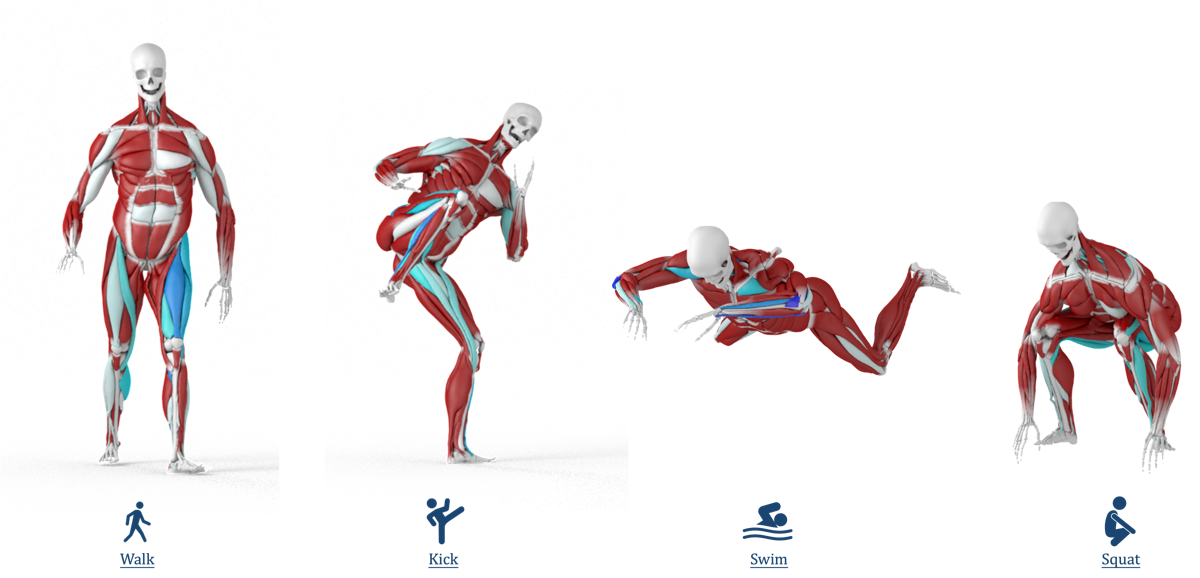
\includegraphics[width=0.78\linewidth]{../images/rlmuscle_preview.png}
  \caption{RLMuscle: reinforcement-learned per-muscle activations drive a 194-muscle volumetric body through walking, kicking, swimming, and squatting at 18\,ms per frame (under review, IEEE TVCG).}
\end{figure}

\section{Future Research Directions}

I see three concrete threads I could start on from day one, and two longer-term visions behind them. What I ultimately want to work on is the bridge between AI, physics, and numerical methods, and that bridge carries traffic in both directions. In \emph{AI for physics}, learning is used to accelerate, generalize, and extend what simulators can already do. In \emph{physics for AI}, the established methods of PDE theory, fluid mechanics, and numerical analysis are turned on learning itself, treating learning dynamics as a system to be understood rather than a procedure to be tuned.

\textbf{1. Next-generation multilevel and Krylov solvers for volumetric deformable bodies.} MGPBD applies linear multigrid to a globally linearized constraint system; I want to go beyond that in two directions. First, \textbf{nonlinear multigrid (FAS)}: a Full Approximation Scheme that operates directly on the nonlinear system, so that coarse levels solve coarse \emph{nonlinear} problems rather than linearized ones. For hyperelastic volumetric bodies under large deformation this avoids repeated global linearization, promises better global convergence behavior, and is a natural fit for constraint-based formulations like XPBD. Second, \textbf{Krylov subspace recycling for spectral reuse}: deformable simulation solves a slowly varying sequence of linear systems, yet standard solvers discard everything between steps. Deflation and recycling techniques, which carry approximate near-kernel and low-end Ritz vectors from one solve to the next, would generalize the lazy prolongator reuse in MGPBD into a principled framework for amortizing spectral information across time steps and frames. Frictional contact is the natural stress test for both ideas, and the reason is structural: contact turns the global solve into a non-smooth complementarity problem whose active set changes every step, which is exactly where naive hierarchy reuse breaks down. Coarse spaces that respect the active contact set, and recycled subspaces that survive contact-set changes, are the two open questions I would most like to attack.

\textbf{2. Contact and friction for robotics: differentiable, robust, and fast enough to be useful.} Contact is where simulation is still least trustworthy, and it is the bottleneck for robotics. Rigid-body contact solvers are fast but resolve geometry crudely; accurate deformable contact is too slow to sit inside a control or design loop; and the non-smoothness of Coulomb friction makes gradients through contact either wrong or uselessly noisy, which is precisely why sim-to-real transfer degrades on contact-rich manipulation. I want to work on all three fronts, building on the recent literature on primal/dual descent methods for dynamics, robust signed-distance-field collision, and continuous collision detection. Concretely: (i) \emph{high-fidelity contact between deformable and articulated bodies}, coupling my GPU multigrid-XPBD solver to rigid multibody dynamics so that soft grippers, tissue, and cables can be simulated in contact-rich scenes without stiffness-induced blowups (my work on real-time cutting is directly relevant here, since both topology changes and contact-set changes destroy the static structure that fast parallel solvers rely on); (ii) \emph{well-behaved contact gradients}, studying how smoothing, relaxation, or randomized-smoothing schemes trade bias against gradient usability, so that differentiable contact becomes a dependable tool rather than a fragile one; and (iii) \emph{learning from contact-rich data}, calibrating friction and contact parameters from real robot interaction in the spirit of real2sim work. The application I find most compelling is programming cable-driven soft robots through differentiable simulation, where what decides whether a design works is contact between the robot and its environment, not just the robot's own deformation.

\textbf{3. The full muscle inverse problem: from video to activations.} My most ambitious concrete goal is to invert the RLMuscle pipeline: instead of generating motion from activations, recover \emph{activations from observation}, estimating what a real person's muscles are doing directly from ordinary video. The forward chain is activations $\to$ volumetric muscle deformation $\to$ skin surface $\to$ image; making the whole chain differentiable turns this into a solvable inverse problem, and each link is now within reach of existing methods. First, an \textbf{ML deformer as a 3D deformation surrogate}: a learned model, trained on data from my high-fidelity muscle simulator, that maps activations and pose to volumetric deformation orders of magnitude faster than the solver and, crucially, is differentiable by construction. This is the surrogate-pyramid idea from RLMuscle, now serving inversion rather than control. Second, \textbf{differentiable rendering} to close the loop against real pixels, the same mechanism already used to program cable-driven soft robots and to calibrate soft-body simulation from depth observations. Third, \textbf{differentiable simulation} as the physical regularizer and the final validator: the surrogate makes the search tractable, while the physically grounded solver keeps solutions anatomically admissible and verifies the recovered activations. The inverse problem is severely ill-posed, since many activation patterns explain the same silhouette, so the interesting research is in the priors: sparsity and co-activation structure, physiological activation dynamics, and consistency with contact forces where the body touches the world. A working version would matter well beyond animation, giving markerless, non-invasive estimates of internal muscle activity for biomechanics, rehabilitation, and sports science.

\textbf{Long-term vision I, AI for physics: learned operators as a way of solving PDEs.} The goal on this side is to let learning accelerate, generalize, and extend classical numerical methods rather than replace them. Neural operators such as DeepONet and Fourier neural operators learn solution \emph{operators} rather than individual solutions, and the ambition behind ``physical foundation models'' is to pretrain across geometries, materials, and boundary conditions so that a new problem needs adaptation rather than training from scratch. I find this direction compelling but, as it currently stands, oversold, and for reasons that are methodological as much as technical. Reported speedups are too often measured against weak baselines rather than against well-implemented classical solvers: a systematic review of the fluid PDE literature found that 79\% of papers claiming to outperform a standard numerical method compared against a weak one.\footnote{N.~McGreivy and A.~Hakim, ``Weak baselines and reporting biases lead to overoptimism in machine learning for fluid-related partial differential equations,'' \emph{Nature Machine Intelligence}, 2024. \url{https://arxiv.org/abs/2407.07218}} Demonstrations also concentrate on toy settings: simple domains, one fixed set of boundary conditions, a narrow band of material parameters. Generalization across boundary conditions, across settings, and above all to genuinely complex geometry is where these methods still fall down, which is precisely the regime that deformable and contact-rich simulation lives in. I believe the productive path is hybrid, and that a solver background is what makes it possible. A learned operator does not have to be the whole solver. It can be a component with a well-defined numerical role: a preconditioner, a coarse-level solve or a learned prolongation inside a multigrid hierarchy, an initial guess for a Newton or Krylov iteration, or a closure model for unresolved scales. In each of these the surrounding iterative solver retains the error control, and the network only has to be approximately right. Two of my assets fit this program directly. My solvers are data engines that can generate large, well-controlled corpora of deformable, contact-rich, and active-material dynamics, the kind of data physical foundation models need and mostly lack. My multigrid work gives me a concrete place to put learned components where their errors are measurable and correctable. This is the version of the neural-operator program I find worth pursuing: simulation as a data engine for learning, and learned components placed only where a solver can still check them.

\textbf{Long-term vision II, physics for AI: studying learning dynamics with the methods of physics.} The mathematics that governs solver convergence also governs learning itself, and in the long run this is the interface I most want to work on. Learning is a dynamical system in its own right, and several of its central puzzles are ones that PDE theory, fluid mechanics, and numerical analysis already have a language for. A recent manifesto for this program calls it ``learning mechanics'': tractable limits, macroscopic laws, hyperparameter theories, and universal behaviors, studied with the habits of physics rather than of engineering practice.\footnote{J.~Simon, D.~Kunin, A.~Atanasov, B.~Bordelon, J.~Cohen, A.~Jacot et al., ``There Will Be a Scientific Theory of Deep Learning,'' 2026. \url{https://arxiv.org/abs/2604.21691}} Neural Tangent Kernel theory shows that gradient descent on wide networks behaves as a kernel method whose convergence per mode is set by the kernel's eigenspectrum, and the resulting spectral bias, where networks learn low-frequency structure first, is precisely the phenomenon multigrid was invented to overcome in iterative solvers. That analogy suggests multilevel and preconditioned training schemes that attack slow-converging modes directly instead of waiting for them. The edge-of-stability behavior of gradient descent, where training settles at the largest step size the local curvature admits, is the learning-rate analogue of the stability limit of an explicit time integrator. Hyperparameter transfer across model scale, where the parameterization is chosen so that settings tuned on small models remain valid on large ones, plays the role that dimensionless numbers play in physics, letting a measurement made at one scale be trusted at another. And spectral properties of the kernel offer a route to explaining scaling laws rather than only fitting them. I want to bring the spectral and dynamical tools of this tradition to bear on understanding and accelerating learning, and to treat optimizer design with the same rigor as time-integrator design.
\end{document}
